%\paragraph{brief}"Histogram of Oriented Gradients" is a popular technique to discover shapes within an image. How it work is by sampling subregions of the image using a kernel. It then checks the slope aka orientation gradient and puts it in a bin. Then it samples another region until entire image been sampled. It then looks in the bin and tries to determine a consensus of slopes to determine where the edges are.
It generalizes the object representation in a way that the output representation for the same object wouldn’t undergo much change under different conditions (like light or other noise), this is called \textbf{feature descriptor}.
It takes input image of object (face in our case) and produces Output vector representing histograms of gradients.\newline It calculates gradient vector for each pixel by measuring change in pixel value along x-direction and y-direction. \newline \newline \textbf{\textit{For example:}}\newline
\begin{figure}
    \centering
	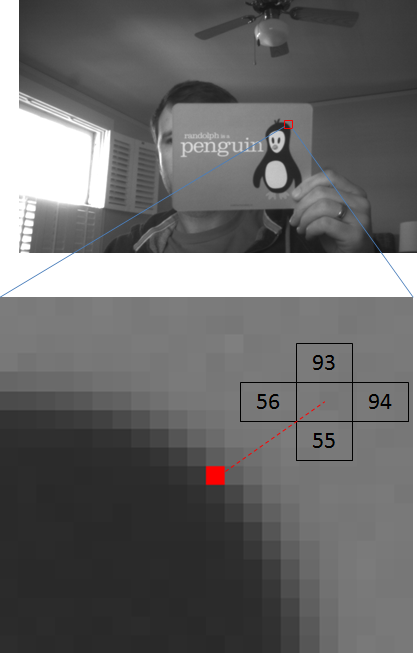
\includegraphics[width=0.3\textwidth]{images/hog_pixel_ex.png}
	\caption{calculating gradient}
	\label{fig:calculating gradient}
\end{figure}
In Figure ~\ref{fig:calculating gradient} this is a grayscale image, so the pixel values just range from 0 (black) : 255 (white), we compute the change in x-direction as the difference in color values between pixels to left and right of current pixel, so in this case it would be 38 ($94 - 56$), note that the subtraction can be from left to right or from right to left but which ever order we take we must use it for the entire image, similarly the change along y-direction is computed as 38 ($93 - 55$), and Now we have our gradient vector:
\[ \begin{bmatrix}
38\\
38\\
\end{bmatrix} \]
The gradient vector for current pixel can be represented with the given magnitude and direction.
\newline \newline
\begin{math}
\mathit{Magnitude} = 
\sqrt{38^2 +  38^2} = 53.47 \newline Angle = arctan(\frac{38}{38}) = 0.785 rad = 45 \degree.
\end{math}
\newline \newline
The angles are between 0 and 180 degrees instead of 0 to 360 degrees. These are called \textbf{“unsigned” gradients} because a gradient and its negative are represented by the same numbers, we don’t use the 0 – 360 degrees because Empirically unsigned gradients work better than signed gradients.
\newline
We can now draw this vector as an arrow on the image and this operation is applied to each pixel in the image. (see figure ~\ref{fig:pixel representation})

\begin{figure}
	\centering
	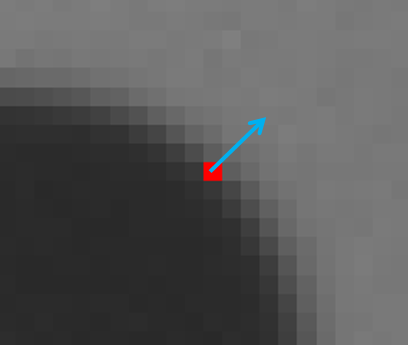
\includegraphics[width=0.5\textwidth]{images/gray_scale.png}
	\caption{a pixel represented by an arrow}
	\label{fig:pixel representation}
\end{figure}
\paragraph{Combining histogram}
We distribute the gradient vectors on n bins to construct a histogram (n can be either 8, 9, 12, …) and we choose n which give us better accuracy.\newline If we have 9 bins, they will be carrying the angles (0, 20, 40, 60, 80, 100, 120, 140, 160). \newline We use histogram with n = 8, the histogram will be formed with angles on horizontal axis and magnitude on vertical axis.
\newline For each gradient vector, its contribution to the histogram is given by the magnitude of the vector (so stronger gradients have a bigger impact on the histogram), We split the contribution between the two closest bins, for example, if a gradient vector has an angle of 85 degrees, then we add
\begin{math}
    \frac{1}{4}
\end{math} 
of its magnitude to the bin centered at 70 degrees, and 
\begin{math}
    \frac{3}{4} 
\end{math}
of its magnitude to the bin centered at 90.
\paragraph{How it’ll be applied on the image?}We divide the image into cells of (1X1, 4X4, …..) and we choose the number of pixels per cell according to which give us the best accuracy.\newline
We use 12X12 pixels per cell.\newline Now we have multiple histogram for a single image we combine them sequentially in a vector. (see figure ~\ref{fig:hist representation})
\begin{figure}
	\centering
	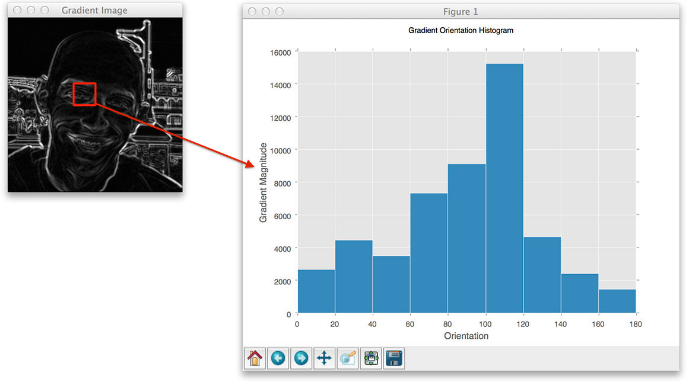
\includegraphics[width=0.5\textwidth]{images/histogram_ex.png}
	\caption{image with part of its histogram}
	\label{fig:hist representation}
\end{figure}
\paragraph{Normalization}
Let’s take a moment to first look at the effect of normalizing gradient vectors in general.
By normalizing your gradient vectors, you can make them invariant to \textit{multiplications} of the pixel values (different illumination conditions)\newline \newline \textbf{\textit{For example:}} \newline
\begin{figure}
	\centering
	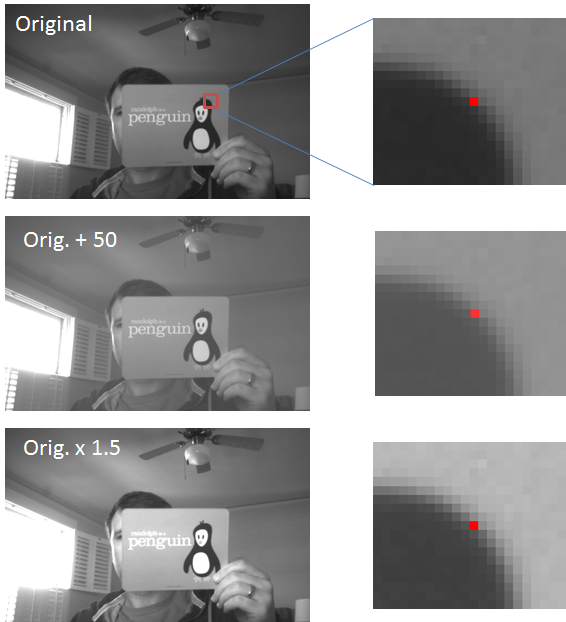
\includegraphics[width=0.5\textwidth]{images/normalization_ex.png}
	\caption{the same image under different conditions}
	\label{fig:normalization}
\end{figure}
In figure ~\ref{fig:normalization} notice how the third image displays an increase in contrast. \newline
The effect of the multiplication is that bright pixels became much brighter while dark pixels only became a little brighter, thereby increasing the contrast between the light and dark parts of the image. 
\newline \newline Let’s look at the actual pixel values and how the gradient vector changes in these three images. \newline The numbers in the boxes below represent the values of the pixels surrounding the pixel marked in red. (see figure ~\ref{fig:normalization calc})
\begin{figure}
	\centering
	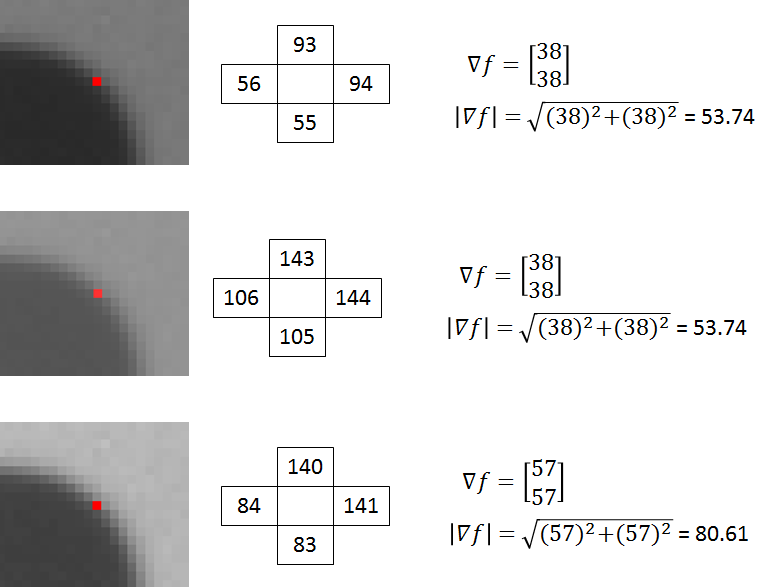
\includegraphics[width=0.5\textwidth]{images/normalization_calc.png}
	\caption{magnitude and angle are calculated in each image}
	\label{fig:normalization calc}
\end{figure}
The gradient vectors are equivalent in the first and second images, but in the third, the gradient vector magnitude has increased by a factor of 1.5. \newline
If you divide all three vectors by their respective magnitudes, you get the same result for all three vectors:
:\[ \begin{bmatrix}
0.71\\0.71
\end{bmatrix} \]
\newline
By dividing the gradient vectors by their magnitude, we can make them invariant (or at least more robust) to changes in contrast. (normalizing to unit length)
\newline Normalizing a vector does not affect its orientation, only the magnitude.
\paragraph{Histogram normalization} Rather than normalize each histogram individually, the cells are first grouped into blocks and normalized based on all histograms in the block, Each block consists of nXn (4X4 in our case) cells 50\% overlapping, the effect of the block overlap is that each cell will appear multiple times in the final descriptor but normalized by a different set of neighboring cells.For more understanding of how the concept of block is applied, see figure ~\ref{fig:block normalization}
\begin{figure}
	\centering
	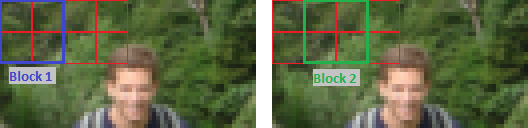
\includegraphics[width=0.5\textwidth]{images/blocks.png}
	\caption{2X2 cells per block, 50\% overlapping}
	\label{fig:block normalization}
\end{figure}
There are four built-in methods, each one is represented by an equation.
\newline We choose L2\_norm by try and error.\newline
All chosen parameter except block normalization according to \cite{hog}.